\documentclass[10pt]{standalone}
\usepackage{commands}

\begin{document}
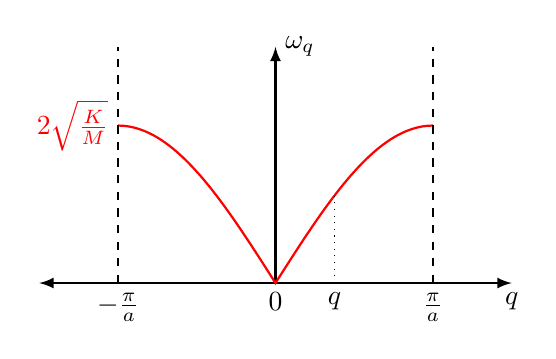
\begin{tikzpicture}
    \draw[-latex, thick] (0, 0) -- (0, 3);
    \draw[latex-latex, thick] (-3, 0) -- (3, 0);
    \node[below] at (3, 0) {$q$};
    \node[right] at (0, 3) {$\omega_q$};
    \draw[red, thick] (-2, 2) cos (0, 0) sin (2, 2);
    \draw[dashed] (-2, 0) -- (-2, 3);
    \draw[dashed] (2, 0) -- (2, 3);
    \node[left, red] at (-2, 2) {$2\sqrt{\frac{K}{M}}$};
    \node[below] at (0, 0) {0};
    \node[below] at (-2, 0) {$-\frac{\pi}{a}$};
    \node[below] at (2, 0) {$\frac{\pi}{a}$};
    \draw[dotted] (0.75, 0) -- (0.75, 1.15);
    \node[below] at (0.75, 0) {$q$};
\end{tikzpicture}
\end{document}